\chapter{实证结果}
\section{定价结果}
按照第4章的Black-Scholes模型\ref{bs-call}和\ref{bs-put},对每个期权的每条交易数据,将距离到期期限、数据期的波动率估计(采用滚动估计方式)、利率、当日比特币价格、行权价等信息输入模型,得到Black-Scholes模型定价。期权的真实价格为当天的成交量加权均价。在定价过程中,我们发现部分期权由于深度价外、而且期限较短,几乎没有模型价值,但仍有较高的真实价格,如果用二者数值的绝对差异将无法表现出这种定价差异的真实影响,损失过多的信息,故定义定价偏差为真实价格与模型价格之比即真实价格/模型价格。同时根据参考文献,深度价外期权和期限较短的期权并不适合用B-S模型定价\cite{10.2307/1831029}\cite{Jame-1979}。因此我们对数据做如下清理:
\begin{itemize}
    \item 剔除每日交易量仅有1的记录
    \item 剔除距离到期日在7日之内的记录
    \item 剔除认购期权的相对价值在0.8以下,认沽期权的相对价值在1.25以上的记录
    \item 剔除期权价格不在期权价格合理范围内的记录,这些期权无法按照价格求得隐含波动率。
\end{itemize}
保留共计600条记录。
600条记录的定价偏差的描述性统计以及按认购、认沽期权的分组统计之后结果如下:
~\\
\begin{center}
    \begin{threeparttable}[H]
    
        \begin{small}
            \caption{定价偏差描述统计}
            \label{tab:option_bias_group}
                \begin{tabular}{lrrr}
\toprule
{} &    定价偏差 &  认购期权定价偏差 &  认沽期权定价偏差 \\
\midrule
count & 600.000 &   364.000 &   236.000 \\
mean  &   0.869 &     0.735 &     1.075 \\
std   &   0.526 &     0.289 &     0.711 \\
min   &   0.105 &     0.105 &     0.282 \\
25\%   &   0.614 &     0.537 &     0.739 \\
50\%   &   0.786 &     0.720 &     0.909 \\
75\%   &   0.997 &     0.886 &     1.162 \\
max   &   5.843 &     2.453 &     5.843 \\
\bottomrule
\end{tabular}

                
        \end{small} 
    \end{threeparttable}
\end{center}
可见在合理的相对价值区间内,真实价格和模型价格差异仍然较大,最大接近6倍。最小接近十分之一,平均水平低于1,说明总体真实价格略低于模型价格。分组结果中,认购期权的平均偏差低于1,而认沽期权的平均偏差高于1,说明平均情况下,认购期权通常价格被低估,而认沽期权通常价格被高估。
~\\
为了初步展示定价偏差和期权价值程度之间的关系,我按照期权的相对价值(比特币价格/行权价)和期限分组,统计了各个组内定价偏差的平均值,以下是定价绝对偏差分组统计的结果:
~\\
\begin{center}
    \begin{threeparttable}[H]
        \centering
        \begin{small}
            \caption{定价偏差分组统计}
            \label{tab:option_bias_group}
                \begin{tabular}{lrrrrr}
\toprule
time\_cut &  0, 30 &  30, 60 &  60, 180 &  180, 624 &  mean \\
moneyness\_cut &          &           &            &             &       \\
\midrule
0.0, 0.6    &    1.027 &     1.126 &      1.075 &       1.129 & 1.109 \\
0.6, 0.9    &    0.822 &     0.968 &      0.911 &       1.029 & 0.937 \\
0.9, 1.1    &    0.812 &     0.774 &      0.953 &       1.102 & 0.843 \\
1.1, 3.9    &    1.010 &     1.054 &      1.016 &       1.185 & 1.063 \\
mean          &    0.856 &     0.903 &      0.961 &       1.098 &       \\
\bottomrule
\end{tabular}

                \begin{tablenotes}
                    \footnotesize
                    \item 注:money\_cut指期权价值程度分组边界(比特币价格/行权价),time\_cut指距到期期限分组边界。
                    
                \end{tablenotes}
        \end{small}
    \end{threeparttable}
        
\end{center}
~\\
可以看到,定价偏差随期限的上升呈增长趋势。对认购和认沽期权分别分组统计,结果如下:
~\\
\begin{center}
    \begin{threeparttable}[H]
        \begin{small}
            \caption{定价偏差分组统计:认购期权}
            \label{tab:call_option_bias_group}
                \begin{tabular}{lrrrrr}
\toprule
time\_cut &  0, 30 &  30, 60 &  60, 180 &  180, 624 &  mean \\
moneyness\_cut &          &           &            &             &       \\
\midrule
0.0, 0.6    &          &     1.167 &      1.073 &       1.129 & 1.113 \\
0.6, 0.9    &    0.789 &     0.964 &      0.891 &       1.027 & 0.924 \\
0.9, 1.1    &    0.769 &     0.725 &      0.806 &       0.932 & 0.770 \\
1.1, 3.9    &    0.937 &     1.032 &      0.875 &       0.941 & 0.939 \\
mean          &    0.797 &     0.870 &      0.911 &       1.063 &       \\
\bottomrule
\end{tabular}

        \end{small}
    \end{threeparttable}
        
\end{center}
~\\
认沽期权分组统计结果:
~\\
\begin{center}
    \begin{threeparttable}[H]
        \begin{small}
            \caption{定价偏差分组统计:认沽期权}
            \label{tab:put_option_bias_group}
                \begin{tabular}{lrrrrr}
\toprule
time\_cut &  0, 30 &  30, 60 &  60, 180 &  180, 624 &  mean \\
moneyness\_cut &          &           &            &             &       \\
\midrule
0.0, 0.6    &    1.027 &     1.003 &      1.104 &             & 1.042 \\
0.6, 0.9    &    0.981 &     1.011 &      1.137 &       1.045 & 1.035 \\
0.9, 1.1    &    0.880 &     0.924 &      1.155 &       1.303 & 0.975 \\
1.1, 3.9    &    1.058 &     1.058 &      1.051 &       1.302 & 1.115 \\
mean          &    0.951 &     0.997 &      1.107 &       1.234 &       \\
\bottomrule
\end{tabular}

    
        \end{small}
    \end{threeparttable}
        
\end{center}
~\\
从分组结果直观而言,对认沽期权实值期权的偏差要小于虚值期权,而对于认购期权这一现象并不明显。
\section{隐含波动率}
隐含波动率即使得Black-Scholes模型价格等于真实价格的波动率参数,这一数值表示了隐含于期权市场价格中与波动率有关的信息。以期权相对价值(S/K)将全部期权分为五组,并求各组平均隐含波动率,以各组相对价值中位数为横轴,隐含波动率为纵轴绘制折线图如下:
\begin{figure}[H]
    \begin{small}
        \begin{center}
            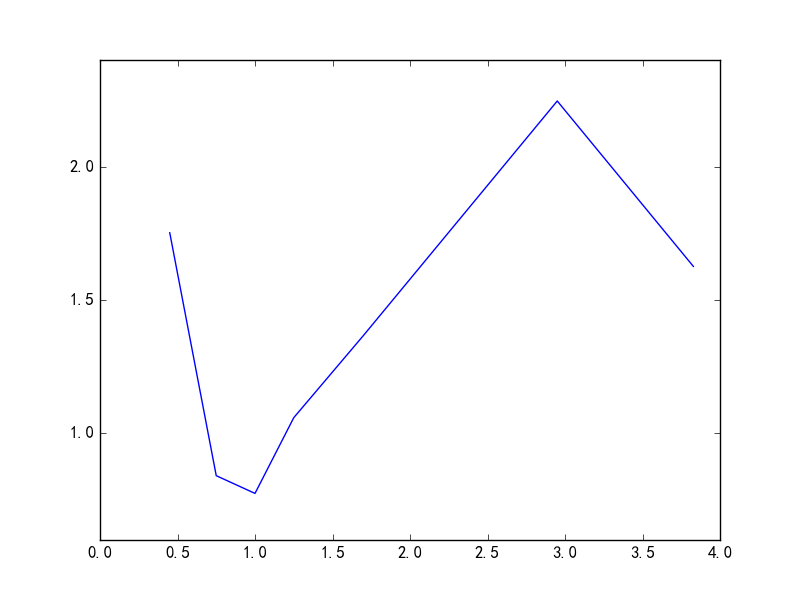
\includegraphics[width=0.95\textwidth]{figures/mean_isd.png}
        \end{center}
        \caption{隐含波动率分组曲线}
        \label{fig:mean_isd}
    \end{small}
\end{figure}
图像呈现出一定的“波动率微笑”性质,相对价值接近1的时候隐含波动率水平更低。本质上隐含波动率微笑现象反映了收益分布与对数正态分布之间的差异。为此我们可以构建两个在回归模型中需要用到的变量。
\par{
    波动率溢价:定义为从现在至期权到期日期间比特币波动率与期权隐含波动率之差。由于波动率越大,一般期权的价格越高,这一指标衡量了期权交易者对波动率的预测与未来期权波动率符合程度。
}
\par{
    在波动率曲面上的斜率:即在图\ref{fig:mean_isd}中,一个期权交易记录的价值程度所在线段的斜率。
}
\section{回归模型}
我们首先构建第\ref{reg vars}节提出的变量,并对其进行描述性统计。变量的描述统计和相关性矩阵如下:
\newpage
\newgeometry{top=1cm,bottom=1cm
}
\begin{landscape} 
    \begin{table}[H]
        \caption{解释变量的描述性统计}
        \resizebox{\linewidth}{!}{
        \begin{tabular}{lrrrrrrrrrrrrrrrrr}
\toprule
{} &  log\_ret &  volatility &  skewness &  amihud &  maxmin\_ratio &  btc\_volume &   time &  const\_delta\_5 &  vol\_pre &  spread &  open\_interest &  slope &  volume &  contract\_is\_call &  inter\_call\_money &  inter\_put\_money &  inter\_call\_skewness \\
\midrule
count &   577.00 &      577.00 &    577.00 &  577.00 &        577.00 &      577.00 & 577.00 &         577.00 &   577.00 &  577.00 &         577.00 & 577.00 &  577.00 &            577.00 &            577.00 &           577.00 &               577.00 \\
mean  &    -0.00 &        0.04 &     -0.39 &    0.04 &          1.04 &       22.45 &   3.75 &           0.14 &     0.01 &  272.88 &          62.84 &   0.00 &   19.48 &              0.60 &              0.58 &             0.41 &                -0.24 \\
std   &     0.05 &        0.02 &      0.76 &    0.02 &          0.03 &        0.40 &   1.00 &           0.47 &     0.02 &  430.01 &          99.58 &   0.00 &   29.35 &              0.49 &              0.50 &             0.51 &                 0.61 \\
min   &    -0.17 &        0.01 &     -4.50 &    0.01 &          1.00 &       21.30 &   2.08 &          -1.00 &    -0.06 & -225.00 &           0.00 &  -0.00 &    2.00 &              0.00 &              0.00 &             0.00 &                -4.50 \\
25\%   &    -0.03 &        0.03 &     -0.81 &    0.03 &          1.01 &       22.16 &   3.09 &          -0.31 &    -0.00 &  121.50 &           9.00 &  -0.00 &    3.00 &              0.00 &              0.00 &             0.00 &                -0.40 \\
50\%   &     0.00 &        0.04 &     -0.23 &    0.04 &          1.03 &       22.36 &   3.56 &           0.36 &     0.01 &  174.00 &          31.00 &   0.00 &    7.00 &              1.00 &              0.86 &             0.00 &                -0.00 \\
75\%   &     0.02 &        0.05 &      0.03 &    0.05 &          1.05 &       22.65 &   4.39 &           0.53 &     0.02 &  310.75 &          98.00 &   0.00 &   20.00 &              1.00 &              0.95 &             0.98 &                 0.00 \\
max   &     0.23 &        0.09 &      1.15 &    0.09 &          1.19 &       23.89 &   6.36 &           1.00 &     0.11 & 9000.00 &        1109.00 &   0.00 &  226.00 &              1.00 &              3.83 &             1.25 &                 1.03 \\
\bottomrule
\end{tabular}

        }
    \end{table}
    \begin{table}[H]
        \caption{解释变量的相关性矩阵}
        \resizebox{\linewidth}{!}{\begin{tabular}{lrrrrrrrrrrrrrrrrr}
\toprule
{} &  log\_ret &  volatility &  skewness &  amihud &  maxmin\_ratio &  btc\_volume &  time &  delta\_5 &  vol\_pre &  spread &  open\_interest &  slope &  volume &  contract\_is\_call &  inter\_call\_money &  inter\_put\_money &  inter\_call\_skewness \\
\midrule
log\_ret             &     1.00 &        0.02 &      0.13 &    0.03 &         -0.12 &       -0.01 &  0.05 &     0.09 &    -0.14 &   -0.02 &          -0.01 &   0.06 &   -0.02 &              0.03 &              0.05 &            -0.00 &                 0.08 \\
volatility          &     0.02 &        1.00 &      0.29 &    0.98 &          0.64 &        0.75 &  0.20 &     0.08 &     0.27 &    0.35 &          -0.20 &   0.07 &   -0.14 &             -0.13 &             -0.11 &             0.14 &                 0.23 \\
skewness            &     0.13 &        0.29 &      1.00 &    0.35 &          0.07 &        0.17 &  0.10 &     0.10 &     0.15 &    0.13 &           0.03 &   0.03 &   -0.06 &              0.01 &              0.05 &             0.00 &                 0.80 \\
amihud              &     0.03 &        0.98 &      0.35 &    1.00 &          0.61 &        0.71 &  0.19 &     0.08 &     0.27 &    0.33 &          -0.20 &   0.07 &   -0.15 &             -0.14 &             -0.11 &             0.15 &                 0.29 \\
maxmin\_ratio        &    -0.12 &        0.64 &      0.07 &    0.61 &          1.00 &        0.64 &  0.15 &     0.06 &    -0.02 &    0.35 &          -0.21 &   0.06 &   -0.13 &             -0.10 &             -0.04 &             0.10 &                 0.07 \\
btc\_volume          &    -0.01 &        0.75 &      0.17 &    0.71 &          0.64 &        1.00 &  0.14 &     0.09 &     0.17 &    0.36 &          -0.17 &   0.10 &   -0.10 &             -0.09 &             -0.03 &             0.10 &                 0.14 \\
time                &     0.05 &        0.20 &      0.10 &    0.19 &          0.15 &        0.14 &  1.00 &     0.17 &     0.21 &    0.32 &           0.02 &  -0.08 &   -0.02 &              0.15 &             -0.08 &            -0.12 &                 0.01 \\
delta\_5             &     0.09 &        0.08 &      0.10 &    0.08 &          0.06 &        0.09 &  0.17 &     1.00 &    -0.15 &    0.16 &          -0.00 &  -0.08 &    0.03 &              0.81 &              0.85 &            -0.73 &                -0.13 \\
vol\_pre             &    -0.14 &        0.27 &      0.15 &    0.27 &         -0.02 &        0.17 &  0.21 &    -0.15 &     1.00 &    0.20 &           0.07 &  -0.05 &   -0.02 &             -0.12 &             -0.18 &             0.10 &                 0.13 \\
spread              &    -0.02 &        0.35 &      0.13 &    0.33 &          0.35 &        0.36 &  0.32 &     0.16 &     0.20 &    1.00 &          -0.10 &   0.02 &   -0.08 &              0.02 &              0.20 &            -0.03 &                 0.10 \\
open\_interest       &    -0.01 &       -0.20 &      0.03 &   -0.20 &         -0.21 &       -0.17 &  0.02 &    -0.00 &     0.07 &   -0.10 &           1.00 &  -0.13 &    0.37 &              0.21 &              0.07 &            -0.20 &                -0.01 \\
slope               &     0.06 &        0.07 &      0.03 &    0.07 &          0.06 &        0.10 & -0.08 &    -0.08 &    -0.05 &    0.02 &          -0.13 &   1.00 &   -0.08 &             -0.42 &             -0.30 &             0.48 &                 0.16 \\
volume              &    -0.02 &       -0.14 &     -0.06 &   -0.15 &         -0.13 &       -0.10 & -0.02 &     0.03 &    -0.02 &   -0.08 &           0.37 &  -0.08 &    1.00 &              0.13 &              0.08 &            -0.12 &                -0.09 \\
contract\_is\_call    &     0.03 &       -0.13 &      0.01 &   -0.14 &         -0.10 &       -0.09 &  0.15 &     0.81 &    -0.12 &    0.02 &           0.21 &  -0.42 &    0.13 &              1.00 &              0.85 &            -0.97 &                -0.28 \\
inter\_call\_money    &     0.05 &       -0.11 &      0.05 &   -0.11 &         -0.04 &       -0.03 & -0.08 &     0.85 &    -0.18 &    0.20 &           0.07 &  -0.30 &    0.08 &              0.85 &              1.00 &            -0.82 &                -0.19 \\
inter\_put\_money     &    -0.00 &        0.14 &      0.00 &    0.15 &          0.10 &        0.10 & -0.12 &    -0.73 &     0.10 &   -0.03 &          -0.20 &   0.48 &   -0.12 &             -0.97 &             -0.82 &             1.00 &                 0.27 \\
inter\_call\_skewness &     0.08 &        0.23 &      0.80 &    0.29 &          0.07 &        0.14 &  0.01 &    -0.13 &     0.13 &    0.10 &          -0.01 &   0.16 &   -0.09 &             -0.28 &             -0.19 &             0.27 &                 1.00 \\
\bottomrule
\end{tabular}
    }
    \end{table}    
\end{landscape}

    \newpage
\restoregeometry
其中,log\_ret为当日比特币对数收益率、volatility为30天滚动估计收益波动率、skewness为30天滚动估计收益偏度、amihud为Amihud非流动性指标,maxmin\_ratio为交易所价格最大者与最小者之比,btc\_volume为当日比特币交易量,time为期权期限,delta\_5为当前模型下计算出的delta,
vol\_pre为波动率溢价(参见\ref{reg vars}),open\_interest为当日该期权持仓量,slope为当日期权波动率曲线的倾斜程度,contract\_is\_call为指示变量,指期权是否为认购期权。
\par{其中,相对价值(比特币价格/行权价)的意义与期权的种类有关,对于认购期权,这一指标越高证明期权价值程度越深,对于认沽期权则完全相反,故构建两个交互变量inter\_call\_money和inter\_put\_money来表示不同类期权中的相对价值对定价偏差的影响。}
\par{从相关性矩阵可见,部分变量之间的相关性水平较高。可利用后向逐步回归的方法剔除部分变量,即先采用全部变量进行回归,再通过AIC信息熵损失最小法逐步选择去掉的变量并进行回归。最终,结合相关性矩阵并参考后向逐步回归结果,可以剔除掉比特币波动率、偏度、期权种类指示变量和偏度的交互项这几个变量。以偏差为解释变量,进行最小二乘法回归,结果如下:}
\newpage
\newgeometry{top=1cm}
\begin{center}
    \begin{threeparttable}[H]

        \caption{回归估计结果}
        \begin{tabular}{lc}
\hline
                   &    定价偏差     \\
\midrule
\midrule
Intercept          & -5.8095***  \\
                   & (1.2262)    \\
log\_ret           & 0.4303      \\
                   & (0.3276)    \\
kurtosis           & 0.1946***   \\
                   & (0.0290)    \\
amihud             & 4.1291***   \\
                   & (1.2595)    \\
maxmin\_ratio      & 0.7072      \\
                   & (0.8066)    \\
btc\_volume        & 0.2097***   \\
                   & (0.0600)    \\
delta\_5           & 0.0847      \\
                   & (0.1568)    \\
vol\_pre           & 11.2719***  \\
                   & (0.9403)    \\
open\_interest     & -0.0000     \\
                   & (0.0002)    \\
slope              & -0.0008     \\
                   & (0.0315)    \\
contract\_is\_call & 0.7138**    \\
                   & (0.2886)    \\
inter\_call\_money & -0.2749**   \\
                   & (0.1140)    \\
inter\_put\_money  & 0.7044***   \\
                   & (0.2508)    \\
observations       & 577.0000    \\
R-Squared          & 0.5975      \\
Adjusted R-Squared & 0.5889      \\
\hline
\end{tabular}
        
        \begin{tablenotes}
            \footnotesize
            \item *:p值<0.1, **:p值<0.05, ***:p值<0.001
            \item 括号中汇报估计系数的标准差。
        \end{tablenotes}
    \end{threeparttable}
\end{center}
\newpage
\restoregeometry
\par{
实际上,这里的定价差异相当于是假设B-S模型价格为供需平衡状态下的均衡价格,而偏差主要衡量了期权的供需不均衡的程度。这些解释变量都能起到解释期权供需差异的意义。峰度为比特币的收益分布与对数正态分布不符的衡量,其系数显著为正,证明了过高的尾部风险会推高期权的价格。比特币的交易量衡量了短期市场的热度,当市场投资情绪较高时,对对冲的要求也更高,故此时对期权的需求更大,提升了期权的价格。衡量比特币交易流动性的Amihud指标、最大价格与最小价格之比两个变量均与比特币市场的流动性有负相关关系,而在回归结果中对期权定价的相对偏差有显著正向关系。说明很可能随着比特币市场流动性下降,投资者对于用期权进行风险管理和投机交易的需求也在不断提升,另一方面,流动性的变差导致B-S模型推导过程中用到的delta-对冲模式不能完整实现,故而导致价格不能回到有效情况下的水准。对于和期权自身性质有关的变量,其中比较显著的影响是波动率溢价。波动率溢价变量本身用到了未来信息,但它能够证明,部分价格看上去过高的期权交易可以被认为是投资者获得了对于未来波动率会更高的信息。除此之外,在控制其他变量不变的情况下,看涨期权价格会相对偏离更高,一般认为看涨期权未来收益上限更高,同时在比特币市场上可能存在更多通过看涨期权进行投机的力量,更高的需求让看涨期权获得了相对更高的交易价格。而对于期权价值程度的交互变量而言,对于两种期权都是实值程度越深,定价偏差越小,这也符合股票市场上观察到的结果。整个模型的R方达到50$\%$以上,有一定的解释能力。
}
\par{为了识别除了价值程度之外,其他变量是否在不同种类的期权中有不用的作用,将两种期权分组之后分别做最小二乘法回归,结果如下:}
\newpage
\newgeometry{top=3cm}
\begin{center}
    \begin{threeparttable}[H]

        \caption{回归估计结果}

        \begin{tabular}{lcc}
\hline
                   &   �Ϲ���Ȩƫ��   &    �Ϲ���Ȩƫ��    \\
\midrule
\midrule
Intercept          & -1.7605*   & -17.8168***  \\
                   & (0.9617)   & (2.9802)     \\
log\_ret           & -1.4445*** & 2.7104***    \\
                   & (0.2854)   & (0.7118)     \\
amihud             & 10.0761*** & 6.2093**     \\
                   & (1.0310)   & (2.9473)     \\
maxmin\_ratio      & 0.2213     & 4.3309***    \\
                   & (0.6263)   & (1.6215)     \\
btc\_volume        & 0.0850*    & 0.6400***    \\
                   & (0.0484)   & (0.1451)     \\
const\_delta\_5    & 0.0966     & 0.6517***    \\
                   & (0.0766)   & (0.2016)     \\
vol\_pre           & 6.1960***  & 8.7675***    \\
                   & (0.8137)   & (2.5295)     \\
spread             & -0.0000    & -0.0003      \\
                   & (0.0000)   & (0.0002)     \\
open\_interest     & -0.0001    & -0.0002      \\
                   & (0.0001)   & (0.0008)     \\
slope              & 4.3934     & 328.7515     \\
                   & (53.8981)  & (251.0568)   \\
observations       & 346.0000   & 231.0000     \\
R-Squared          & 0.6172     & 0.5472       \\
Adjusted R-Squared & 0.6069     & 0.5287       \\
\hline
\end{tabular}
        \begin{tablenotes}
            \footnotesize
            \item *:p值<0.1, **:p值<0.05, ***:p值<0.001
            \item 括号中汇报估计系数的标准差。
        \end{tablenotes}
    \end{threeparttable}
\end{center}
\newpage
\restoregeometry
将认购期权和认沽期权分别回归后,可以发现很多变量对于两者有着不同的效应。
\section{套利策略}
将第\ref{strategy}节构建的策略应用到筛选后的数据上。一个普通的delta套利策略结果如下所示(分call和put描述):
~\\
\begin{tabular}{lr}
\toprule
{} &    认购期权收益 \\
\midrule
个数 &     76.00 \\
平均值  &   5090.33 \\
t-值   & 3.40 \\
胜率 & 69.74\%\\
min   & -22514.80 \\
50\%   &   2612.82 \\ 
max   &  39066.98 \\
\bottomrule
\end{tabular}

\begin{tabular}{lr}
\toprule
{} &    认购期权收益 \\
\midrule
count &     56.00 \\
mean  &   5853.38 \\
std   &  29050.16 \\
min   & -29224.75 \\
25\%   &  -4621.06 \\
50\%   &     79.32 \\
75\%   &   9984.46 \\
max   & 175590.24 \\
\bottomrule
\end{tabular}

~\\
对于认购期权,大部分期权都能获得较高的正向收益,而认沽期权则不能,可见认沽期权的定价误差可能更多地由于整体市场对期权需求维持在较高水平,导致其定价本身存在很高溢价,简单的B-S模型不能反映其真实价格。而用模型对认购期权定价则包含了一定的信息成分,能够被用于套利操作。
% 采用第\ref{strategy}节介绍的最优对冲法则构建策略,得到的结果如下所示(分call和put描述):
% ~\\
% \begin{tabular}{lr}
\toprule
{} &             0 \\
\midrule
count &     76.000000 \\
mean  &   5104.506291 \\
std   &  24053.321740 \\
min   & -54736.735804 \\
25\%   &  -2544.558660 \\
50\%   &   1296.627105 \\
75\%   &  14581.982485 \\
max   &  95924.759292 \\
\bottomrule
\end{tabular}

% \begin{tabular}{lr}
\toprule
{} &              0 \\
\midrule
count &      56.000000 \\
mean  &    5807.606247 \\
std   &   28789.975974 \\
min   &  -28960.119116 \\
25\%   &   -4713.496122 \\
50\%   &      78.646932 \\
75\%   &    8878.368538 \\
max   &  171978.145231 \\
\bottomrule
\end{tabular}

% ~\\